% コンパイル方法: lualatex filename.tex
\RequirePackage{plautopatch}

\documentclass[a4paper, 10pt]{ltjsarticle}


% マージン設定
\usepackage[top=20mm, bottom=20mm, left=20mm, right=20mm]{geometry}

% LuaLaTeX用日本語対応パッケージ
\usepackage{luatexja}
\usepackage{luatexja-fontspec}

% 必要なパッケージ
\usepackage{fontspec}
\usepackage{titlesec}
\usepackage{graphicx}
\usepackage{amsmath}
\usepackage{hyperref}
\usepackage[english, japanese]{babel}
\usepackage{multicol} % 二段組用パッケージ
\usepackage{indentfirst}
\usepackage{tikz} % カスタム点線用
\usepackage{authblk} % 著者・所属パッケージ
\usepackage{here}
\usepackage{caption}
\setmainfont[Ligatures=TeX]{Times New Roman}
\setmainjfont[BoldFont=MS Gothic]{MS Mincho}

\renewcommand{\baselinestretch}{0.95}

% セクション見出しのカスタマイズ
\titleformat{\section}
  {\fontsize{10pt}{10pt}}
  {\thesection.}
  {1em}{}


\setlength{\parindent}{1em}
% \setlength{\belowcaptionskip}{1em} % キャプション下の余白を -10pt に設定



\titlespacing*{\section}{0em}{1em}{0em}


\pagestyle{empty}


\begin{document}

\setlength{\columnsep}{7.5mm}

\twocolumn[
    \begin{center}
        {\vspace{-1em}}

        {\fontsize{15pt}{15pt}\selectfont{クロスレイヤシミュレータ開発における無線LANシミュレータの開発}}

        {\vspace{1.5em}}

        {\fontsize{13pt}{13pt}\selectfont{ Development of a CSMA/CA Simulator in the Context of an Integrated Simulator Spanning from the Physical Layer to the MAC Layer }}
    \end{center}



    \begin{flushright}
      {\fontsize{11pt}{11pt}\selectfont{T5-16 下沢亮太郎\\}}
      {\fontsize{11pt}{11pt}\selectfont{指導教員 設樂勇}}
    \end{flushright}

    \vspace{1em}

    \thispagestyle{empty}
]

\section{緒言}
近年,無線通信端末利用者の急増に伴い様々な場所で無線通信システムが利用されており、今後も利用の増加と発展が見込まれている.


\section{提案手法}


\section{結果}

\begin{figure}[h]
  \centering
  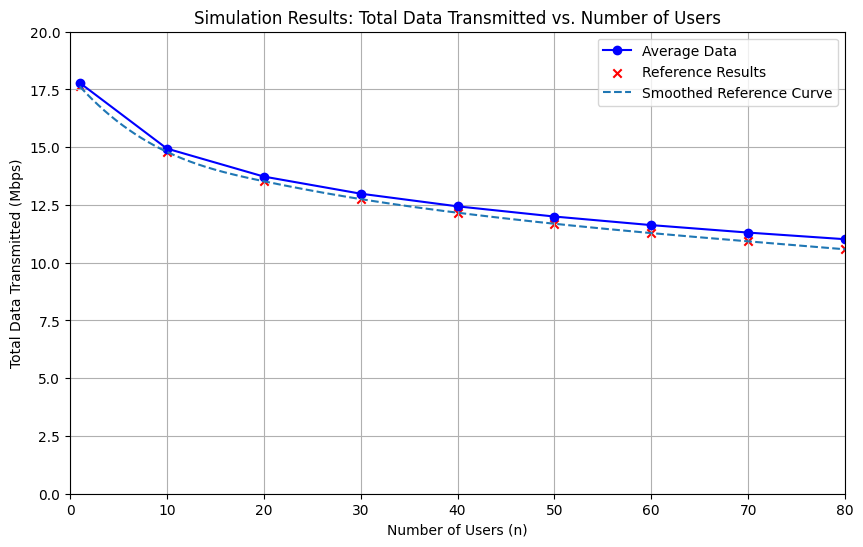
\includegraphics[width=0.8\columnwidth]{./assets/graph.png}
\end{figure}

\section{結言}


\end{document}
